\pagestyle{fancy}
%\newpage
\chapter{PSI: PLANIFICACIÓN DEL SISTEMA DE INFORMACIÓN}

	\vspace{2cm}	
	\begin{center}
	{\Large \textbf{FASE DE PLANIFICACIÓN} \par}
	\end{center}
	\vspace{5cm}
	
	\begin{center}
	\Huge \textbf{PSI}\par
	\end{center}

\newpage

\section{PSI 1: INICIO DEL PLAN DE SISTEMAS DE INFORMACIÓN}

\subsection{PSI 1.1: Análisis de la Necesidad del PSI} 
El tutor de este trabajo de fin de grado, José Manuel Redondo, ha propuesto el desarrollo de una aplicación web para el Museo de la Informática de Asturias, que contenga toda la información disponible sobre los componentes del museo y la muestre de forma ordenada para que las personas interesadas puedan acceder a ella fácilmente. El sistema será gestionado directamente por el tutor del trabajo.
\par El sistema debe identificar cada componente y mostrar la información disponible del mismo,. El software permitirá añadir la información de las nuevas piezas que puedan ser incluidas en la exposición en un futuro gracias a donaciones o compras. Los componentes serán ordenados según su tipo y la época a la que pertenecen. 

\subsection{PSI 1.2: Identificación del Alcance del PSI}
Actualmente los carteles informativos sobre las piezas del museo se encuentran expuestos en la Escuela de Ingeniería Informática. Los objetivos de este proyecto son los siguientes:
\begin{itemize}
	\item Recopilar los datos disponibles de las piezas que se encuentran actualmente en el Museo e introducirlos en una base de datos.	
	\item Mostrar una linea temporal con los diferentes periodos a los que pertenecen los componentes del Museo. 
	\item Permitir acceder a cada periodo para ver los componentes del mismo.
	\item Organizar las diferentes piezas en función de su tipo y de la familia de la que forman parte.
	\item Presentar la información disponible de cada pieza, así como imágenes de la misma y otras curiosidades.
\end{itemize}
En definitiva, estos objetivos se pueden resumir en:
\begin{itemize}
	\item Permitir a los usuarios visitar el Museo de la Informática de forma online, ofreciendo la misma información que se encuentra disponible en la exposición física.
	\item Facilitar al administrador la inserción de nuevos periodos y componentes.
\end{itemize}

\subsection{PSI 1.3: Determinación de Responsables}
\begin{itemize}
	\item \textbf{El proyectante} se encargará del desarrollo del software descrito y de realizar la carga de los datos disponibles a la base de datos correspondientes.
	\item\textbf{El tutor del proyecto} se encargará de la supervisión de las fases del proyecto y de su validación.
	\item \textbf{Una serie de usuarios escogidos aleatoriamente} realizará pruebas del software para comprobar su correcto funcionamiento.
\end{itemize}


%\newpage
%\section{PSI 2: DEFINICIÓN Y ORGANIZACIÓN DEL PSI}
% 
%
%\subsection{PSI 2.1: Especificación del Ámbito y Alcance} 
%
%
%\subsection{PSI 2.2: Organización del PSI}


%\newpage
%\section{PSI 3: ESTUDIO DE LA INFORMACIÓN RELEVANTE}
% 
%\subsection{PSI 3.1: Selección y Análisis de Antecedentes} 


\newpage

\section{PSI 7: DEFINICIÓN DE LA ARQUITECTURA TECNOLÓGICA}
%\subsection{PSI 7.1: Identificación de las Necesidades de Infraestructura Tecnológica} 


\subsection{PSI 7.2: Selección de la Arquitectura Tecnológica} 
Al tratarse de una aplicación Angular, seguirá el patrón Modelo Vista Vista-Modelo (MVVM), una variación del Modelo Vista Controlador, patrón arquitectónico que separa los datos y la lógica de una aplicación de su representación. En la variación MVVM, la vista y el modelo son muy dependientes entre sí. \par 
En este caso la vista estará compuesta por las \textit{templates} de Angular, que son componentes HTML.\par
El modelo se corresponde con la base de datos MySQL y a la que se accede desde un servidor Apache que aloja los archivos PHP necesarios.\par
Por último, la vista-modelo es la propia aplicación de Angular.
\begin{figure}[H]
\centering
\centerline{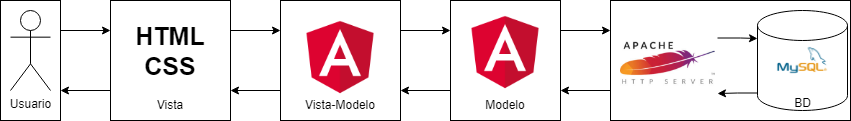
\includegraphics[scale=0.6]{arq-tec}}
\caption{Diagrama de la arquitectura tecnológica}
\end{figure}